%% %%%%%%%%%%%%%%%%%%%%%%%%%%%%%%%%%%%%%%%%%%%%%%%%%%%%%%%%%%%%%%%%%%%%%%%%%%%
%%
%%    author(s): RoboCupAtHome Technical Committee(s)
%%  description: Introduction - Leagues
%%
%% %%%%%%%%%%%%%%%%%%%%%%%%%%%%%%%%%%%%%%%%%%%%%%%%%%%%%%%%%%%%%%%%%%%%%%%%%%%
\section{Leagues}
\label{sec:leagues}

\iterm{RoboCup@Home} is divided in three Leagues. Two of them are \Term{Standard Platform League}{SPL}s for which all competitors use the same robot, and one that grants complete freedom to all competitors. The official leagues and their names are:
\begin{itemize}
  \item the \Term{RoboCup@Home Domestic Standard Platform League}{RoboCup@Home DSPL},
  \item the \Term{RoboCup@HomeSocial Standard Platform League}{RoboCup@Home SSPL}, and
  \item the \Term{RoboCup@Home Open Platform League}{RoboCup@Home OPL}
\end{itemize}

\begin{wrapfigure}[21]{r}{0.30\textwidth}
	\centering
	\vspace{-30pt}
	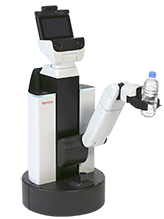
\includegraphics[width=0.25\textwidth]{images/toyota_hsr.png}
	\vspace{-10pt}
	\label{fig:toyotaHSR}
	\caption{Toyota HSR}
	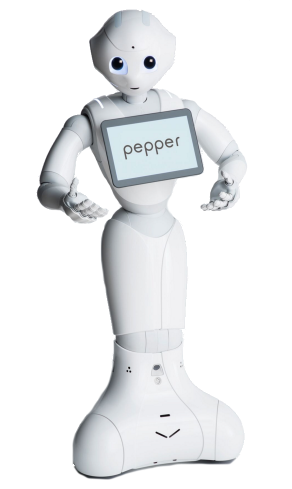
\includegraphics[width=0.20\textwidth]{images/softbank_pepper.png}
	\vspace{-10pt}
	\label{fig:softbank-pepper}
	\caption{Softbank / Aldebaran Pepper}
\end{wrapfigure}
Each league points out to a different aspect of service robotics, reason for which they target specific abilities.


\subsection{Domestic Standard Platform League}
The \iterm{Domestic Standard Platform League}(DSPL) has as main goal to assist humans in a domestic environment, paying special attention to elderly people and people suffering of illness or disability. In consequence, the DSPL focuses on Ambient Intelligence, Computer Vision, Object Manipulation, Safe Indoor Navigation and Mapping, and Task Planning.

The robot to be used in the DSPL is the Toyota HSR, shown in Figure \ref{fig:toyota-hsr}.

\subsection{Social Standard Platform League}
With a 180 degree turn in Human Robot Interaction, the \iterm{Social Standard Platform League}(SSPL) takes robots away from the traditional passive servant role, for now the robot is the one who will actively look for interaction. From a party waiter in a home environment to a hostess in a museum or shopping mall, in \iterm{SSPL} look for the next user who may require its services. Hence, this league focuses on Human-Robot Interaction, Natural Language Processing, People Detection and Recognition, Reactive Behaviors, and Safe Outdoor Navigation and Mapping.

The robot to be used in the SSPL is the Softbank/Aldebaran Pepper, shown in Figure \ref{fig:softbank-pepper}.

\subsection{Open Platform League}
The \iterm{Open Platform League}(OPL) has the same modus operandi used since the fundation of RoboCup@Home till 2017 when Standard Platform Leagues were created. With no hardware constrains, OPL is the league for teams who want to test their own robot designs and configuration, as well as for old at-homers. In this league robots are tested to their limits without having in mind design restriction, although the scope is similar to the DSPL. 